\section{ Overview of the algorihtm }
The following section will describe how the algorithm works in general.
Firstly, it will specify the problem statement. 
After that, it will describe a short mathematical explanation. 
Then, it will sketch out the steps of the algorithm.

\subsection{Problem statement}

Given an NxN hamiltonian matrix $A$ and $\vec a$ vector $\vec b$, we want to solve for the vector $\vec x$ such that,
\begin{equation}
A \vec{x} = \vec{b}
\end{equation}
To solve for x the equation can be rewritten as
\begin{equation}
\vec{x} = A^{-1}\vec{b}
\end{equation}
Note that to encode $\vec b$ we need $\mathcal{O}(log_2 N)$ qubits.

As described earlier the hermitian matrix $A^{-1}$ can be split into its spectral decomposition. 
$A$ can be represented in terms of its eigenvalues $U_1 ... U_n$ and eigenvectors $\lambda_1 ... \lambda_n$.
\begin{equation} 
A =  U D U^{\dagger} = \begin{pmatrix} U_1 & ...& U_n \end{pmatrix} \begin{pmatrix} \lambda_1 & 0 & 0 \\  0 & \ddots & 0\\ 0 & 0& \lambda_n \\ \end{pmatrix} \begin{pmatrix} U^\dagger_1 \\ ...\\ U^\dagger_n \end{pmatrix}
\end{equation}

This means, if we can find the eigenvalues and eigenvectors of $A$ we can then solve the linear equation quite easily. 
Classical solutions involving spectral decomposition are not faster than other standard algorithms such as Gaussian Elimination. 
Though, estimating eigenvalues and eigenwerte can be performed quite efficiently by quantum methods.
Via amplitude amplification, QPE can be accelerated to generate the eigenvalues and eigenvectors in $\mathcal{O}(log_2 N)$ steps.

In the quantum version the linear equation looks like this
\begin{equation}
\ket{x} = A^{-1}\ket{b}
\end{equation}
where $\ket b$ and $\ket x$ are the quantum state of the $\vec b$ and $\vec x$ vectors respectively.
Note that  $\ket x$ is just a quantum state. 
We can not read every element to achieve the vector $\vec x$. 
So far we were able to perform everything in $\mathcal{O}(log_2 N)$.
Reading out every entry of $\vec x$ would take $\mathcal{O} (N)$ steps which would destroy our speed up.
But, as we are only interested in an approximation, we can compute an expectation value $\bra x M \ket x$, where $M$ is some linear operator. 
With this method we can extract many statistical features like normalization, distribution of weights, moments, etc.



\subsection{Mathematical Overview}
We will now look at a mathematical overview of what is happening in the quantum circuit.
We will also assume that the matrix $A$ is hermitian. If $A$ is not hermitian, we can write $A$ as a hermitian like this

\begin{equation}
A^\dagger = \begin{pmatrix} 0 & A \\ \overline{A^T}& 0 \end{pmatrix}
\end{equation}

As already mentioned the matrix can now be described as a linear combination of its outer products of its eigenvectors and its eigenvalues.
In the quantum version the formula looks like this

\begin{equation}
A = \sum_{i=0}^{N-1} \lambda_i \ket{u_i}\bra{u_i}
\end{equation}
where $\ket u_i  \bra u_i$ are the outer products of $A$ and $\lambda_i$ are the eigenvalues of $A$. 
$N$ is the size of the matrix $A$.
We can rewrite the formula for the inverse $A^{-1}$ as such

\begin{equation}
A^{-1} = \sum_{i=0}^{N-1} \lambda_i^{-1} \ket{u_i}\bra{u_i}
\end{equation}

Similary $\ket b$ can be expressed in the eigenbasis of $A$ like this
\begin{equation}
\ket{b} = \sum_{j=0}^{N-1} b_j\ket{u_j}
\end{equation}

We now have all the tools to solve the equation by inserting the definition of $A^{-1}$ and $\ket b$ into our original equation,
\begin{align*}
\ket{x} &= A^{-1} \ket{b}\\
&=\left(\sum_{i=0}^{N-1} \lambda_i^{-1} \ket{u_i}\bra{u_i} \right) \left(\sum_{j=0}^{N-1} b_j\ket{u_j} \right) \\
&=\sum_{i=0}^{N-1} \sum_{j=0}^{N-1} \lambda_i^{N-1} \ket{u_i}\bra{u_i} b_j\ket{u_j}\\
&=\sum_{i=0}^{N-1} \sum_{j=0}^{N-1} \lambda_i^{-1} b_j\ket{u_i}\braket{u_i| u_j}\\
&=\sum_{i=0}^{N-1} \sum_{j=0}^{N-1} \lambda_i^{-1} b_j\ket{u_i}\delta_{ij}\\
&=\sum_{i=0}^{N-1} \lambda_i^{-1} b_j\ket{u_j}\\
\end{align*}
As we can see we can encode the solution $\ket x$ of our linear system into our quantum system quite nicely.
That means, $\ket x$ can be calculated, only by determinining the eigenvectors and eigenvalues of A. 
Using Quantum Phase Estimation, calculating the eigenvalues and eigenvectors for a unitary $U$ can be very efficient.



\subsection{Quantum Circuit}

\begin{figure}
    \centering
    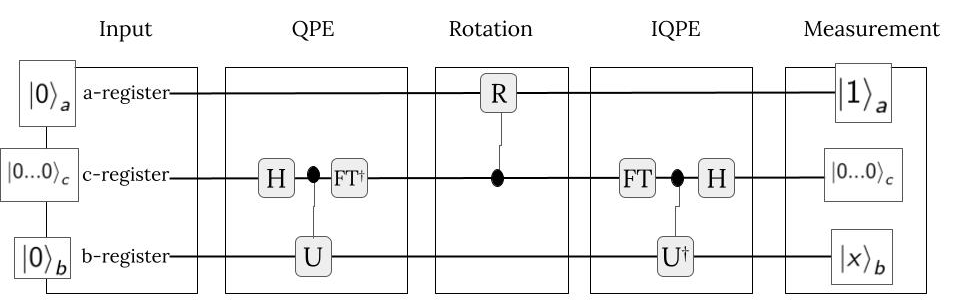
\includegraphics[width=9.0cm]{img/example_circuit_cropped.png}
    \caption{Example Circuit}
    \label{ex_circ}
\end{figure}


We will now look at how the algorithm is implemented in the quantum circuit. 
We will firstly look at the sets of qubits need for the algorithm. 
Then, we will describe the phases of the procedure.

\subsubsection{Registers}
Fig.~\ref{ex_circ} shows the scheme of a simple quantum circuit for the HHL algorithm.
We have three registers which describe three different sets of qubits in the quantum circuit.

The a-register contains the ancilla qubit. 
It is used for the inversion of the eigenvalues and will be explained in detail later on.

The c-register, oftentimes refered to as the clock-register, is used for the quantum phase estimation part. It is related to the time (clock) of the controlled rotation of the qubits and will store the eigenvalues after performing QPE.

The b-register contains the $\vec{b}$ vector which is encoded into a quantum state $\ket{b}$. 
After the whole HHL procedure is done the b-register will contain the solution state $\ket{x}$.



\subsubsection{Phases}
The procedure of the quantum circuit can be split into 5 phases:

\begin{itemize}
\item State preparation
\item Quantum phase estimation (QPE)
\item Inversion of eigenvalues
\item Inverse quantum phase estimation (IQPE)
\item Measurement of $\ket x$
\end{itemize}

In the state preparation phase, the vector $\vec{b}$ will be encoded into a quantum state $\ket{b}$ and the $A$ matrix will be encoded as a hamiltonian, which is a unitary operator
$U=e^{iAt}$ into the QPE and IQPE operations.

The Quantum Phase Estimation will then calculate the eigenvalues and eigenvectors of the A matrix.

Then, we perform the rotation and invert the eigenvalues through rotary operations. 
Unfortunately, these operations have a probability to fail, as they are not unitary operators.
The ancilla will detect wether the rotation was successfull or not.
It will either collapse to $\ket0$ or $\ket1$ for failure and success respectively.
If the rotation is not successfull, the procedure has to be repeated from the beginning. 
If the rotation was successfull we can continue the procedure. 
The problem is, that the qubits in the b-register and c-register are entangled. 
This means that we cannot factorize the result into a tensor product of the c-register and b-register.
As a result, we cannot convert the b-register into the $\ket 0$ / $\ket 1$ measurement basis with the desired amplitudes.
We will need to uncompute the state so that it gives the right results in the $\ket 0$ / $\ket 1$ measurement during which the b-register and c-register will be unentangled.
That means we have undo all operations until now to unentangle the states, keeping the inverted eigenvalues though.

This is achieved by the Inverse Quantum Phase Estimation which undos all steps we performed in the QPE phase, leaving us with the a $\ket{0...0}$ state in the c-register and the $\ket x$ state in the b-register.

Lastly, the $\ket x$ state is to be measured. As mentioned earlier, we can only read out an approximation of an expectation value $\bra x M \ket x$.
